\section{Current-state summaries are insufficient for revisability}
\label{sec:state-only}

The control ladder in Section~\ref{sec:behavior} already showed that the main MHST/Qwen effect survives several current-state checks: matching of designated incumbent/challenger state by construction, the leader-consistent subset, the exact $k{=}0$ null, and the output-margin control. The state-only insufficiency decomposition compresses that logic into one quantitative object: what a simple current-state model predicts from current-state summaries alone, what the actual paired history effect is, and what residual paired effect remains.

We reuse the same mean-flipability target as the companion behavioral summary. For each valid example $e$, $\MeanFlip(e)$ is the mean over doses of the hard flip indicator derived from raw barriers. We then fit a monotone state-only predictor using only designated margin $m$ and prefix-only output margin $\oprefix$, implemented as isotonic regression of $\MeanFlip$ on $\oprefix$ separately for each $m$ using train examples with valid individual semantics. No history type, $k$, pair identifier, latent feature, or intervention-derived quantity enters the model. The paired prediction is simply the difference between the fresh and committed predictions within each held-out test pair.

The result is clean. On held-out paired-valid test pairs, the observed paired mean-flipability gap is $0.3969$ (95\% CI $[0.3420, 0.4510]$), while the state-only predictor accounts for only $0.3531$ ($[0.3121, 0.3946]$), leaving a positive residual paired gap of $0.0439$ ($[0.0131, 0.0756]$). The same pattern remains on the leader-consistent subset, where the residual is $0.0548$ ($[0.0212, 0.0914]$). The null cell behaves exactly as it should: for $k{=}0$, actual, predicted, and residual gaps are all $0.0$, while the pooled $k{>}0$ subset remains positive with residual $0.0592$ ($[0.0178, 0.1016]$).

\begin{figure}[t]
    \centering
    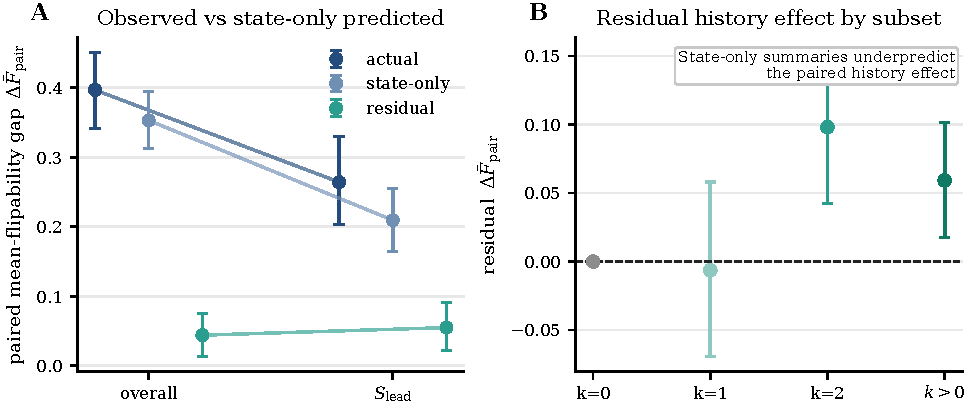
\includegraphics[width=\linewidth]{figures/figure4_state_only_insufficiency.pdf}
    \caption{State-only insufficiency decomposition on held-out MHST/Qwen test pairs. \textbf{A}: actual paired mean-flipability gap, state-only predicted paired gap, and residual paired gap for the overall valid-pair subset and the leader-consistent subset. \textbf{B}: residual paired gap by subset; the $k{=}0$ cell remains exactly null, while $k{>}0$ remains positive. The decomposition therefore shows that current-state summaries underpredict the observed paired history effect.}
    \label{fig:state-only}
\end{figure}

\begin{table}[t]
    \centering
    \small
    \begin{threeparttable}
    \caption{State-only insufficiency decomposition on held-out MHST/Qwen test pairs.}
    \label{tab:state-only}
    \begin{tabularx}{\linewidth}{>{\raggedright\arraybackslash}X c c c c}
        \toprule
        Subset & Pairs & Actual $\DeltaMeanFlip$ & Predicted & Residual \\
        \midrule
        Overall & 185 & 0.3969 [0.3420, 0.4510] & 0.3531 [0.3121, 0.3946] & 0.0439 [0.0131, 0.0756] \\
        Leader-consistent $\Slead$ & 113 & 0.2642 [0.2035, 0.3300] & 0.2094 [0.1645, 0.2550] & 0.0548 [0.0212, 0.0914] \\
        $k{=}0$ & 48 & 0.0000 [0.0000, 0.0000] & 0.0000 [0.0000, 0.0000] & 0.0000 [0.0000, 0.0000] \\
        $k{>}0$ & 137 & 0.5360 [0.4744, 0.5975] & 0.4768 [0.4346, 0.5193] & 0.0592 [0.0178, 0.1016] \\
        \bottomrule
    \end{tabularx}
    \begin{tablenotes}[flushleft]
        \item The state-only model is intentionally narrow: isotonic regression of mean flipability on prefix-only output margin, fitted separately for each designated margin $m$. The residual is therefore the paired history effect not explained by these current-state summaries alone.
    \end{tablenotes}
    \end{threeparttable}
\end{table}

This is the paper's second main result. A simple monotone current-state model built from the two most defensible current-state summaries in the project still underpredicts the paired history effect. That does not make the result latent or causal, but it sharpens the behavioral conclusion: state matching is insufficient for revisability.
